% !Mode:: "TeX:UTF-8"
\documentclass[newgeometry=true,type=doctor]{hithesis}

\usepackage{ltablex}
\usepackage{tikz}
\usepackage{verbatim}
\usetikzlibrary{%
   decorations.fractals%
  ,decorations.pathmorphing%
  ,shadows%
}
\pdfstringdefDisableCommands{%
  \def\heiti{}%
  \def\,{}%
  \def\\{}%
  \def\hspace{}
  \def\ccwd{}
  \def\quad{}
  \def\hskip{}
}
\graphicspath{{figures/}}
\renewcommand{\contentsname}{目 \quad 录}
\renewcommand\bibname{参考文献}

\usepackage{tikz}
\usetikzlibrary{calc}
\usetikzlibrary{shapes,arrows}
\usepackage{amsmath} % nice math symbols
\usepackage{bm} % bold math
\usepackage{color} % change text color
%%%<
\usepackage{verbatim}
%\usepackage[active,tightpage]{preview}
%\PreviewEnvironment{tikzpicture}
%\setlength\PreviewBorder{5pt}%
\usepackage{listings}
%设置代码风格
\definecolor{codegreen}{rgb}{0,0.6,0}
\definecolor{codegray}{rgb}{0.5,0.5,0.5}
\definecolor{codepurple}{rgb}{0.58,0,0.82}
\definecolor{backcolour}{rgb}{0.95,0.95,0.92}

\lstdefinestyle{mystyle}{
    backgroundcolor=\color{backcolour},
    commentstyle=\color{codegreen},
    keywordstyle=\color{magenta},
    numberstyle=\tiny\color{codegray},
    stringstyle=\color{codepurple},
    basicstyle=\footnotesize,
    breakatwhitespace=false,
    breaklines=true,
    captionpos=b,
    keepspaces=true,
    numbers=left,
    numbersep=5pt,
    showspaces=false,
    showstringspaces=false,
    showtabs=false,
    tabsize=2
}
\usepackage{threeparttable}

\begin{document}

\parindent0pt
\null
\thispagestyle{empty}
%\vskip3cm
\vfill
\hfil
%: définition des couleurs et des styles
% fond Gauche et Droite bleu marron
\definecolor{couleurGauche}{rgb}{.25,1,1}
\definecolor{couleurDroite}{rgb}{.75,.5,0.25}
% Post-It jaune
\definecolor{couleurPostIt}{rgb}{.9,.9,.35}
% logo TikZ dégradé blanc gris Top et Bottom
\definecolor{couleurTop}{rgb}{1,1,1}
\definecolor{couleurBottom}{rgb}{.5,.5,.5}



\tikzset{fondA/.style={ball color=couleurGauche}}
\tikzset{fondB/.style={ball color=couleurDroite}}
\tikzset{fondPostit/.style={color= couleurPostIt}}
\tikzset{ombrePunaise/.style={color={blue!10!gray}}}
\tikzset{ombrePostit/.style={color={black},opacity=.5}}
\tikzset{punaise/.style={ball color=red}}

% ============ utilitaires de construction ============
%: \ruban{angle}{point}
\newcommand{\ruban}[2]{\shadedraw[rotate=#1] #2
  ++(0:0.57735*\arete-0.57735*\epaisseur+2*\rayon)
  ++(-30:\epaisseur-1.73205*\rayon)
  arc (60:0:\rayon)   -- ++(90:\epaisseur)
  arc (0:60:\rayon)   -- ++(150:\arete)
  arc (60:120:\rayon) -- ++(210:\epaisseur)
  arc (120:60:\rayon) -- cycle;}

%: \logoTikZ{(point)}{angle}{TikZ}{pour}{L'impatient}
\newcommand{\logoTikZ}[5]
{\def\arete{3}   \def\epaisseur{5}   \def\rayon{2}
\begin{scope} [very thick,top color= couleurTop,bottom color= couleurBottom,rotate=#2]
	\coordinate (a) at ($#1+(0,-6)$);
	\coordinate (b) at ($#1+(6,-6)$);
	\coordinate (c) at ($#1+(6,6)$);
	\coordinate (d) at ($#1+(0,6)$);
	\ruban{0}{#1};
	\ruban{120}{#1};
	\ruban{-120}{#1};
	\draw #1 ++(-60:3.5) node[scale=5,rotate={#2+30}]{#3};
	\draw #1 ++(180:3.5) node[scale=3,rotate={#2-90}]{#5};
	\clip (a) -- (b) -- (c) -- (d) -- cycle; % pour croiser
	\ruban{0} {#1};
	\draw #1 ++(60:3.5) node [gray,xscale=-3,yscale=3,rotate={360-#2+30}]{#4};
\end{scope}}

% un trait épais et trois ovales empilés
%: \epingle{point}{angle}{échelle}
\newcommand{\epingle}[3]{
\coordinate[rotate=#2,yshift={#3*0.375cm}] (e) at #1;
\coordinate[shift={++(60:0.75)}] (g) at (e);
\begin{scope} [scale=1.5]
 \begin{scope}[rotate=-30]
   \coordinate[shift={++(30:0.75)}] (h) at (e);
   \draw[ombrePunaise,line cap=round,line width=4pt] (e) -- ++(60:0.75);
   \fill [ombrePunaise,rotate=-30,scale=0.5] (h) ellipse (.65 and .3) ;
   \fill [ombrePunaise,rotate=60,scale=0.5] (h) ++(0.4,0) ellipse (.4 and .3);
   \fill [ombrePunaise,rotate=60,scale=0.5] (h) ++(0.8,0) ellipse (.2 and .4);
 \end{scope}
 \draw[line cap=round,line width=4pt] (e) -- ++(60:0.75);
 \fill [punaise,rotate=-30,scale=0.5] (g) ellipse (.65cm and .3cm) ;
 \fill [punaise,rotate=60,scale=0.5] (g) ++(0.4,0) ellipse (.4 and .3);
 \fill [punaise,rotate=60,scale=0.5] (g) ++(0.8,0) ellipse (.2 and .4);
\end{scope}}


%: \postIt{(point)}{angle}{échelle}{ligne 1}{ligne 2}{ligne 3}}
\newcommand{\postIt}[6]
{\begin{scope} [rotate=#2]
\fill [red,ombrePostit] #1 ++ ($#3*(-1.45,0.72)$) -- ++ ($#3*(2.86,0)$)
 .. controls+(0,0)and+($#3*(-0.25,0.05)$).. ++ ($#3*(0.25,-2.4)$)
 .. controls+($#3*(-0.1,-0.1)$)and+(0,0).. ++ ($#3*(-2.95,0.1)$)
 -- cycle;
\fill [ombrePostit] #1 ++ ($#3*(-1.45,0.72)$) -- ++ ($#3*(2.86,0)$)
 .. controls+(0,0)and+($#3*(-0.25,0.05)$).. ++ ($#3*(0.2,-2.35)$)
 .. controls+($#3*(-0.1,-0.1)$)and+(0,0).. ++ ($#3*(-2.95,0.1)$)
 -- cycle;
\fill [ombrePostit] #1 ++ ($#3*(-1.45,0.72)$) -- ++ ($#3*(2.86,0)$)
 .. controls+(0,0)and+($#3*(-0.25,0.05)$).. ++ ($#3*(0.15,-2.3)$)
 .. controls+($#3*(-0.1,-0.1)$)and+(0,0).. ++ ($#3*(-2.95,0.1)$)
 -- cycle;
\fill [fondPostit] #1 ++ ($#3*(-1.45,0.72)$) -- ++ ($#3*(2.86,0)$)
 .. controls+(0,0)and+($#3*(-0.2,0.1)$).. ++($#3*(0.1,-2.25)$)
 .. controls+($#3*(-0.1,-0.1)$)and+(0,0).. ++ ($#3*(-2.95,0.1)$)
 -- cycle;
\end{scope}
\epingle{#1}{#2}{#3}
% texte
\draw #1 node [scale=#3,rotate=#2] {#4};
\draw #1 node [scale=#3,rotate=#2,below={#3*0.05cm}] {#5};
\draw #1 node [scale=#3,rotate=#2,below={#3*0.2cm}] {#6};}

% pour un placement précis des divers éléments
\tikzset{ajustage/.style={yshift=0.cm}}

%: ===== PAGE

%: XeLaTeX \font\fantaisie pour sous-titre et texte du Post-It
\font\fantaisie="Lucida Handwriting" at 10pt

\thispagestyle{empty}
%===========================================================================
\begin{tikzpicture}[remember picture,overlay]
% fond bicolore gauche droite
\coordinate [ajustage] (cp) at (current page);
\coordinate [ajustage] (cpe) at (current page.east);
\coordinate [ajustage] (cpne) at (current page.north east);
\coordinate [ajustage] (cpn) at (current page.north);
\coordinate [ajustage] (cpnw) at (current page.north west);
\coordinate [ajustage] (cpw) at (current page.west);
\coordinate [ajustage] (cpsw) at (current page.south west);
\coordinate [ajustage] (cps) at (current page.south);
\coordinate [ajustage] (cpse) at (current page.south east);
\fill[fondA] (cps) .. controls (cpw) and (cpe) .. (cpn) -- (cpnw)  -- (cpsw) -- cycle;
\fill[fondB] (cps) .. controls (cpw) and (cpe) .. (cpn) -- (cpne)  -- (cpse) -- cycle;
\draw[white,line width=4pt] (cps) .. controls (cpw) and (cpe) .. (cpn);
\draw[white,line width=8pt] (cpnw)--(cpne)--(cpse)--(cpsw)--cycle;


% Logo à peu en dessous du centre (bord interne aligné avec la courbe)
\logoTikZ{(cp)}{25}{\scriptsize Notebook}{p{\color{orange}oo}{\color{gray}f}{\color{orange}ee}}{\Large FEM}

% TikZ pour l'impatient en haut à gauche
\draw (cp)  node [xshift=-9.5cm,yshift=12cm,scale=6.5,right] {有{\color{orange}\textit{限元}}};
\draw (cp)  node [xshift=-9cm,yshift=9.1cm,scale=6,right] {\fantaisie 从};
\draw (cp)  node [xshift=-6cm,yshift=9.8cm,scale=3,right] {\fantaisie 入门};
\draw (cp)  node [xshift=-3.8cm,yshift=9.1cm,scale=6,right] {\fantaisie 到};
\draw (cp)  node [xshift=-6cm,yshift=8.6cm,scale=3,right] {\fantaisie 入土};

% Auteurs au centre sous le titre
\draw (cp)  node [xshift=-10cm,yshift=-10cm,scale=4,right,color={red},align=left] {十三飞};
%\draw (cp)  node [xshift=-8.7cm,yshift=6.95cm,scale=2,right,color={purple},align=left] {豆};
%\draw (cp)  node [xshift=-8.23cm,yshift=7.3cm,scale=3,right,color={blue},align=left] {三};
%\draw (cp)  node [xshift=-8.1cm,yshift=7.3cm,scale=4,right,color={violet},align=left] {飞};

% post'it en bas à droite avec les auteurs
\coordinate[xshift=4.5cm,yshift=-9.5cm] (postit) at (cp);
\postIt{(postit)}{17}{1.75} {\fantaisie
stay hungry}{}{\fantaisie stay foolish}
%L\raisebox{0.25\height}{A}T\raisebox{-0.25\height}{E}X et TikZ}


\end{tikzpicture}

\vfill
\parindent4pt

\frontmatter

\pagenumbering{Roman}
\pagestyle{hit@headings}
\setcounter{page}{0}
\tableofcontents    % 中文目录
\newpage

\vspace{9em}

{\songti \yihao \textbf{前\,\,\,\,言}}

\vspace{8em}






\mainmatter
\chapter{软件介绍及使用说明}

\section{整体介绍}

\section{操作说明}

\section{如何获得本软件?}
\chapter{软件编译}
本软件按照如下方式进行编译。
\section{编译所需要工具}
编译之前需要安装的模块有:
\begin{enumerate}
	\item Qtribbon
	\item Qtdock
\end{enumerate}
\subsection{Qt}
需要注意的是,必须是MSVC版本的Qt,因为目前某些库对该编译器有依赖,5.0版本以上理论上都可以编译通过。
\section{编译过程}
使用Qtcreator或者Visual Studio打开feem.pro文件,全部构建即可。
\chapter{模块介绍}
这一章节主要介绍软件的开发过程,将软件按照功能逐步地进行细致划分,从而完成软件的设计任务。
\section{软件框图}
如 \figurename{} \ref{fig:softarch} 为软件整体的关系图。
\begin{figure}[h]
	\centering
	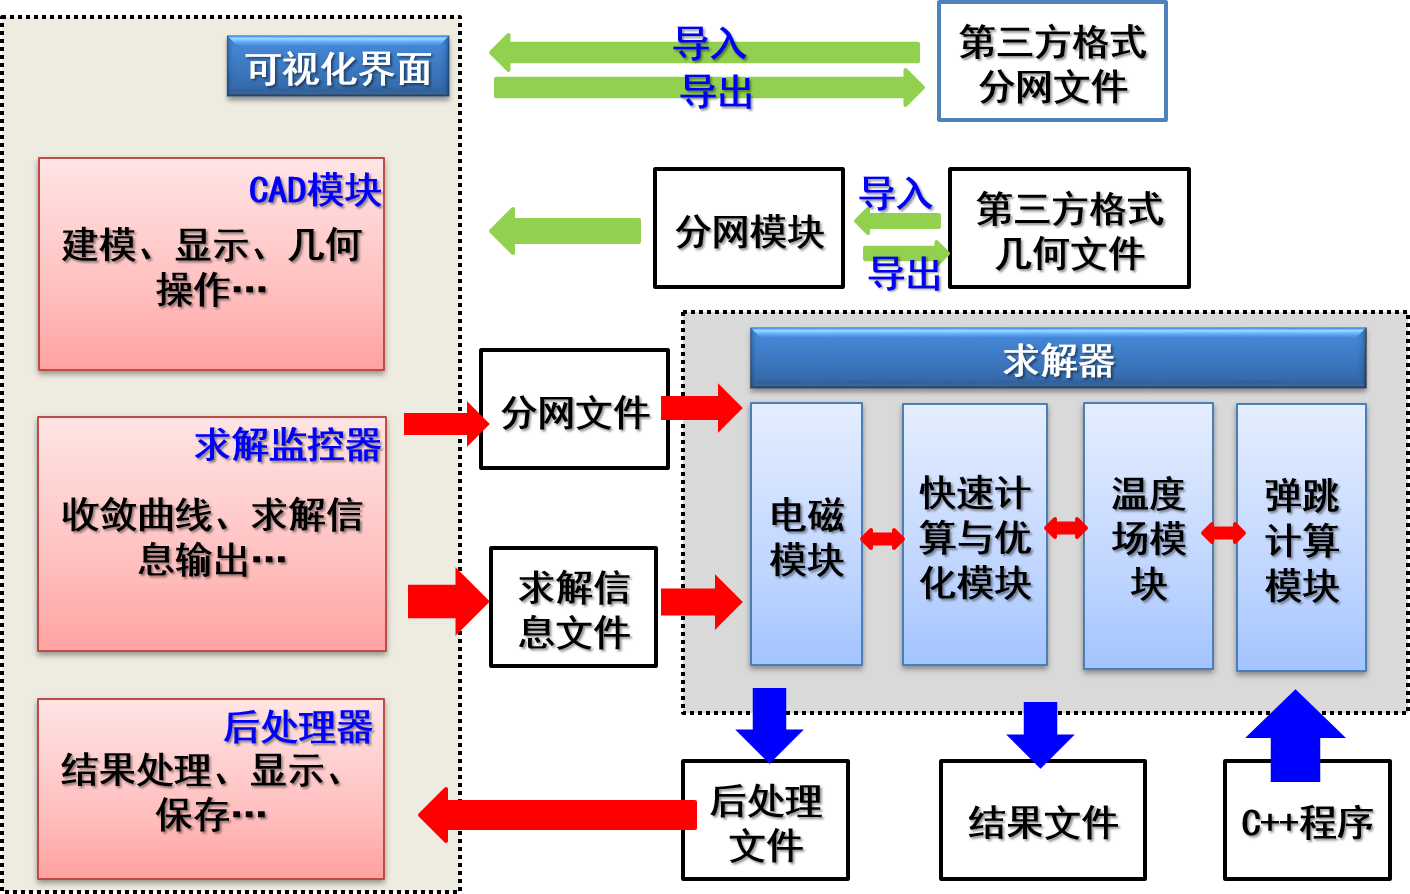
\includegraphics[width=0.7\linewidth]{figures/softarch}
	\caption{软件FEEM整体设计框架}
	\label{fig:softarch}
\end{figure}

\subsection{磁场问题的有限元求解}

\subsubsection{静磁场}

\subsubsection{瞬态磁场}
在电器当中的瞬态问题,主要还是考虑到可动部件的运动。

静态特性

在静态特性计算当中,可运动部件并没有真的在运动。只不过相对固定部分发生一定的位移之后,计算出电磁场的分布。求解的是一组静磁场问题。也没有考虑任何的动态方程,等同于针对位移的参数求解。

动态特性

实际的仿真过程需要考虑运动的耦合。电磁-运动的耦合是一种电磁问题和运动学问题的弱耦合。在每一个时间步的计算当中,先求解电磁场问题,然后再求解运动学问题,求解过程如下:

1.求解麦克斯韦方程组,计算发生一定位移后,施加在运动部件上的电磁力或电磁力矩;

2.求解运动部件的动态方程,计算出运动部件在时间步内的加速度值和速度,并且计算出下一时间步时运动部件新的位移位置;

3.将运动部件移动到新的位置,并且进行重分网操作;

4.返回步骤1。

\subsection{电磁力的计算}

Arkkio’s method


各种方法的优缺点对比

stress tensor方法的缺点

在数学上,这种方法是完全正确的,能够得到准确的力矩值,前提是B的计算值是准确的。然而,通常情况下不是这样的。需要注意的是,有限元求解是一种数值计算方法,因此,我们大多数情况下处理的都是近似值。特别地,我们实际求解得到的是磁势向量A,而磁感应强度B是通过计算A的旋度来得到的。这实际上是一个微分过程,如果我们对某些不准确的变量进行了微分操作,那么最后得到的计算结果必然也是有误差的。也就是说,我们计算得到的B的误差将会比A的误差更大。如果能够取消这个微分计算的过程,那么将有可能提高计算精度。
\subsection{优化问题}

\section{界面设计}

\subsection{Ribbon模块}
Ribbon模块是一个能够提供类似Office界面风格的组件。同时,COMSOL采用的也是类似界面。

1.如何自定义Ribbon的主题?
\subsection{QtFLEX模块}
该模块实现类似Visual studio当中的可停靠用户界面的组件。窗口内部的子部件可以根据用户随意的进行位置放置。可以设置自动隐藏停靠,可以与其他窗口进行分割,合并。
\begin{figure}
	\centering
	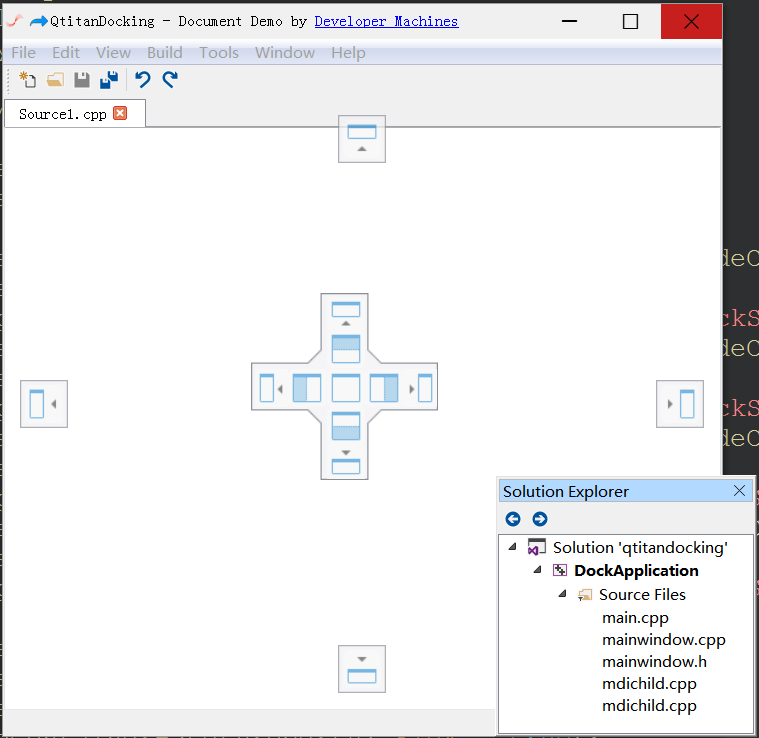
\includegraphics[width=0.7\linewidth]{figures/dock}
	\caption{Dock演示}
	\label{fig:dock}
\end{figure}

\subsection{界面布局}

\section{定义}
为了对数据进行存储,需要定义合理的格式和存储方式。
\subsection{工程文件格式及存储}
工程文件,即是软件会打开的文件,通过读取这个文件,软件可以获得该项目当中的几何模型、物理设置参数、分网信息、求解信息等。目前,最普遍的方式就是采用标记式语言进行存储,首选XML语言。
\subsection{几何文件格式及存储}
几何图形是用户在操作软件过程当中一直会使用到的东西,所以这部分数据肯定是常驻内存。在软件的核心,需要定义几何存储的格式来代表各种图形,这些图形可以是用户自己创建的,也可以是不同格式的几何文件转换过来的。
\subsection{分网文件格式及存储}
跟几何文件类似,也需要在工程内部自定义分网数据格式,来保存从各种格式的分网文件读取并转换而来的数据。
\subsection{结果数据文件及存储}
在求解结束后,需要一个数据结构来存储计算得到的各种数据结果。
\subsection{编程代码规范}
为了使软件开发尽量的规范,开发小组成员应当遵守以下操作:
\section{CAD绘图}
几何绘图是软件可视化最重要的一个部分。
\subsection{绘图原理}
在显示屏上你所看到的有趣的东西,都是程序员尽力地让一切看起来都跟真的似的,实际上,它依旧还是冷冰冰的机器,只是用的时间长了可能会发热而已。
\subsection{基本几何形状}
需要实现的基本几何形状有:点、线、圆弧、长方形等。
\subsection{形状操作}
所谓的用户能够对显示的几何形状进行控制,实际上是程序针对用户的鼠标操作与实际几何形状的位置进行了比较计算之后,进行了一些算法。每一次改变都会导致显示内容的刷新,只不过肉眼无法辨别出来。
\subsubsection{形状选中、调整大小、删除、隐藏显示}

\subsubsection{自动吸附}

\subsubsection{布尔操作}

\subsubsection{缩放、变形}

\subsection{与分网显示、后处理的接口}

\subsection{参数绘图}

\section{材料库}
为了对模型当中的结构添加相应的材料属性,需要提供一个材料管理器的功能,能够存储一些常见的材料,并且能够实现新建、修改、删除等操作。
\subsection{已有材料库}

\subsection{新建、删除材料}

\subsection{导入、导出材料}

\section{分网生成}
分网无疑是有限元器求解最为关键的步骤之一。
\subsection{分网读取、导出}

\subsection{有限元分网形状}

\subsection{读取几何模型并分网}

\subsection{分网控制}

\subsection{删除分网}

\subsection{分网可视化}

\section{求解器}

\subsection{求解器设置}

\subsection{优化模块}
当所有的求解信息都设置好后,不仅可以实现磁场的求解,还能够实现对某些参数的优化设计。

\subsection{收敛曲线显示}

\section{后处理}
求解器计算得到的结果无疑要使用最好的方式展现给用户。
\subsection{结果曲线}

\subsection{结果云图}

\subsection{结果矢量图}

\subsection{数据导出}
\chapter{测试模型}
\chapter{开发问题记录}

\section{开发技巧}   

\subsection{Qt包含目录}
在使用Qt的某一个模块的时候,需要include相应的头文件,为了告诉编译器头文件的具体位置,需要在pro文件中指定需要使用的相关模块,这样qmake会对pro文件进行处理,生成相应的路径。也可以指定不是用某些库。

常见的模块有:core、gui、widgets等,如果想要包含private的头文件,那么就需要接着添加core-private、gui-private、widgets-private等。具体的效果可以使用VS打开pro文件,然后查看相应的头文件设置信息。          

\subsection{预编译文件}
当一个工程项目很大时,会出现很多的头文件,这个时候,把他们全部一次性加入到工程当中是一件非常繁琐和头疼的事情。在Qt当中,可以进行这样的方便设置。将每一个模块的代码(包括h文件和cpp文件)单独放置在一个文件下面,然后再新建一个pri文件,在pri文件当中设置需要include的文件列表。这样,当我们需要使用这个模块时,不需要再把源代码加入到工程当中,只需要把该pri文件include到pro文件当中,这样就可以了。

\subsection{Qtcreator子项目}
在一个较大的工程项目当中,会有多个子项目,同时编译得到最后的文件。这在vs当中被称为solution。qtcreator当中也有类似的功能。

主要的操作是:在顶部的pro文件当中设置模板TEMPLATE为subdirs模式;然后设置SUBDIRS,添加指定的工程模块;使用"CONFIG+=ordered"配置为顺序编译。需要注意的是每一个单独的子项目都需要能够单独编译成功。为了方便,可以将这些工程的目标文件的生成路径设为一致。

这个子项目跟上面的pri文件不同,该文件对应的是一个项目很多时,包含很多模块进行简化。

\subsection{default构造函数}
在C++当中,类里面的数据大部分都是私有的,外部无法访问的,所以需要定义一些函数来进行赋值或者初始化的操作,这些函数可以称为接口。C++的类通过构造函数来对数据进行初始化操作,一个类当中可以有多个构造函数,这些函数的名称跟类名一致。当在类中没有定义任何构造函数时,C++会给你提供一个无参数的默认构造函数。但是,当你定义了一个含有参数的构造函数时,编译器就不再提供这个构造函数,如果你需要使用这个函数,就需要自己自已一个,否则,编译器就会报错。为了减轻程序员的负担,在C++的类声明时,使用"=default"来表示让编译器生成一个默认的构造函数,这样就不需要自己再去实现了。这个构造函数是在类的内部实现的,所以是一个内联函数。但是,vs2013之前的编译器都不支持这种语法,会报错。

需要注意的是,在vs2013当中遇到了这个错误:multiple versions of a defaulted special member functions are not allowed。原因可能是,使用default定义了一个默认构造函数,同时定义了一个含有参数的构造参数,但是这个参数的默认值被设为了null,编译器就认为出现了两个默认构造函数,所以会报错。

\subsection{error LNK2019: unresolved external symbol compress referenced in function}
如果使用Qtcreator出现了这个问题,恰好编译器是vs的话,有可能是一下原因:确定一下在pro文件当中,头文件列表和源文件列表中被调用函数的源文件是不是出现在了调用文件的后面,如果是的话,将它移动到前面去。

\subsection{构造函数}
1.父类没有声明构造函数

(1)子类也没有声明构造函数,则父类和子类均由编译器生成默认的构造函数;

(2)子类中声明了构造函数(无参或者带参),则子类的构造函数可以写成任何形式,不用顾忌父类的构造函数。在创建子类对象时,需要先调用父类的默认构造函数(编译器自动生成),然后再调用子类的构造函数。

2.父类只声明了无参数构造函数

如果子类的构造函数没有明显地调用父类的构造函数,则将会调用父类的无参构造函数。

3.父类只声明了带参数的构造函数

子类的构造函数必须显式得调用父类的构造函数。

4.父类同时声明了无参和有参构造函数

子类的构造函数调用其中一个即可。如果没有显式调用的话,会默认调用父类无参构造函数。

\subsection{Texstudio与sumatrapdf反向搜索关联}

sumatrapdf是一款免费小巧的PDF阅读器,双击PDF的某一个区域,可以打开关联的tex文件的相应位置。对于winedit,"D:/My Program Files/CTEX/WinEdt/WinEdt.exe" "[Open(|\%f|);SelPar(\%l,8)]"
对于TeXstudio"D:/My Program Files/TeXstudio/texstudio.exe"  "\%f" -line \%l

\subsection{VS不同版本编译报错}
出现“无法找到文件MSVCP120D.DLL”的问题,问题在于某些使用的dll文件是vs2013生成的,而现在使用的vs版本不是2013,解决方法就是将这些dll在新的vs下重新编译。

\subsection{Qt国际化}
在软件当中,需要实现界面的中文显示,这里采用的是Qt的国际化方案,也就是提供针对软件界面文字的中国版本的翻译文件,将国家设为中国就可以了。

简单介绍一下实现的步骤(详细的可以参考网上的教程):首先,在你需要翻译的地方,字符串需要写在tr函数当中,然后在pro文件当中加入ts文件,接着运行lupdate命令,生成相应的ts文件;然后使用语言家软件打开ts文件,或者你直接打开ts文件进行编辑,设置好相应的翻译;完成之后,运行lrelease命令生成压缩版的翻译文件qm;然后就是怎么使用的问题了,网上有好几种方案,一种就是放在exe文件的运行目录,另一种就是将qm文件放到工程的资源文件当中,这样的好处就是避免了文件的丢失,别人的篡改等等,可以编译进二进制文件当中。而且,如果加入到资源文件当中,每次自动生成qm文件就还在那个位置,就不需要你把它再拷贝到exe目录里。

简单说一下,在load qm文件时遇到的坑。我已经把qm文件加入到了qrc文件当中,但是无论如何都不能正确的载入,网上搜索了各种教程也不行。qm文件其实也拷贝到了文件夹下,也是不行。后来在res文件夹下面新建了一个translations文件夹,然后qm文件都放在了里面,然后接着load就好使了,我也不知道是为什么。

需要注意的是,如果在不同分支当中同时运行了lupdate来更新翻译,由于ts文件会继续翻译短语的所在文件和行号,所以合并的时候,ts文件可能会出现冲突。可以采用一个不生产行号的方法来折中处理。但是为了避免麻烦,还是在单一的分支当中提交翻译吧。

\subsection{如何保存程序的配置信息?}
在程序的运行过程当中,用户可能会对窗口的位置、大小进行一些改变,或者程序的一些信息做了更改,如何在下次启动时能够保持原样?在Qt当中,是通过配置文件实现的。

\subsection{如何在状态栏上添加一些复杂的控件?}

\subsection{warning: C4819: The file contains a character that cannot}
你的源码是不带BOM的UTF8格式,但是MSVC不知道你用的UTF8。由于你在简体中文Windows系统下,它就认为你用的是GB18030(也叫GB2312,GBK,CP936)。

当你一个汉字时,占3个字节,用GB18030是无法解析的(1个半汉字)。当你2个汉字时,占6个字节,用GB18030碰巧可以解释成3个汉字。

如果不指定的话默认是 utf-8。所以我们用 gcc 时很少关注这个问题。

Viual Stdio 中就麻烦多了。这里先说 Visual stdio 2015,这个是我现在用的编译环境。VS2015 中如果源代码是 utf-8的,执行字符集默认是本地 Locale 字符集,对于简体中文的 windows 系统来说,这个 本地Locale字符集是 gb18030。所以直接显示汉字会全是乱码。解决这个乱码有三个办法,第一个办法是编译时加入命令行参数,在 Qt 的 pro 文件中可以这样:

msvc:QMAKE\_CXXFLAGS += -execution-charset:utf-8
1
第二个办法是在源文件中加入:

\#pragma execution\_character\_set("utf-8")

\subsection{如何制作图标?}
SVG格式的图标怎么制作?适用于什么情况?

\subsection{生成注释}
为了方便阅读源代码,需要自动生成注释。从源代码当中提取注释并生成文档的方案是有的,那就是doxygen,但是一个个去添加固定格式的注释简直很烦诶,还需要自动根据代码当中的函数添加注释模版。这个东西貌似需要IDE支持。

1.doxygen的安装

如果IDE是qtcreator的话,可以安装doxygen的插件,直接去\href{https://github.com/fpoussin/qtcreator-doxygen}{Github qtcreator-doxygen}下载。这个插件的编译需要跟qtcreator的源代码一起编译生成,所以你必须下载对应版本的插件,其实就是一个dll文件。

下载好dll文件后,将其放到qtcreator安装目录下的plugins目录,然后重启就可以了。之后,就会在工具菜单下多了一个doxygen子菜单,然后就可以自动地给整个文件添加注释了。这个注释最好添加在源文件当中。

添加完注释之后,就是利用doxygen生成文档了。

2.doxygen的编译

网上仅提供了某些版本的二进制文件,但是没有最新版,如何编译得到最新版qtcreator的doxygen插件?

\subsection{Paint事件}
导致画面闪烁的关键原因分析:

一、绘制窗口由于大小位置状态改变进行重绘操作时,绘图窗口内容或大小每改变一次,都要调用Paint事件进行重绘操作,该操作会使画面重新刷新一次以维持窗口正常显示。刷新过程中会导致所有图元重新绘制,而各个图元的重绘操作并不会导致Paint事件发生,因此窗口的每一次刷新只会调用Paint事件一次。窗口刷新一次的过程中,每一个图元的重绘都会立即显示到窗口,因此整个窗口中,只要是图元所在的位置,都在刷新,而刷新的时间是有差别的,闪烁现象自然会出现。所以说,此时导致窗口闪烁现象的关键因素并不在于Paint事件调用的次数多少,而在于各个图元的重绘。

根据以上分析可知,当图元数目不多时,窗口刷新的位置也不多,窗口闪烁效果并不严重;当图元数目较多时,绘图窗口进行重绘的图元数量增加,绘图窗口每一次刷新都会导致较多的图元重新绘制,窗口的较多位置都在刷新,闪烁现象自然就会越来越严重。特别是图元比较大绘制时间比较长时,闪烁问题会更加严重,因为时间延迟会更长。
解决上述问题的关键在于:窗口刷新一次的过程中,让所有图元同时显示到窗口。

二、进行鼠标跟踪绘制操作或者对图元进行变形操作时,当进行鼠标跟踪绘制操作或者对图元进行变形操作时,Paint事件会频繁发生,这会使窗口的刷新次数大大增加。虽然窗口刷新一次的过程中所有图元同时显示到窗口,但也会有时间延迟,因为此时窗口刷新的时间间隔远小于图元每一次显示到窗口所用的时间。因此闪烁现象并不能完全消除!所以说,此时导致窗口闪烁现象的关键因素在于Paint事件发生的次数多少。
解决此问题的关键在于:设置窗体或控件的几个关键属性。

解决双缓冲的关键技术:

1、设置显示图元控件的几个属性: 必须要设置,否则效果不是很明显!
this.SetStyle(ControlStyles.OptimizedDoubleBuffer | ControlStyles.ResizeRedraw |ControlStyles.AllPaintingInWmPaint, true);

2、窗口刷新一次的过程中,让所有图元同时显示到窗口。

可以通过以下几种方式实现,这几种方式都涉及到Graphics对象的创建方式。
Graphics对象的创建方式:

a、在内存上创建一块和显示控件相同大小的画布,在这块画布上创建Graphics对象。接着所有的图元都在这块画布上绘制,绘制完成以后再使用该画布覆盖显示控件的背景,从而达到“显示一次仅刷新一次”的效果!

b、直接在内存上创建Graphics对象:

\subsection{MSVC中文注释导致的编译错误}
遇到这个问题是将代码在虚拟机下面进行编译的时候出现的。在另外一台电脑上编译运行没有任何问题,但是在这台电脑上运行就好几百个问题,刚开始也是丈二和尚,后来慢慢领悟到应该又是中文编码的问题导致没有正确的解析源代码。

为什么会出现编码错误呢?主要是中文的存在。编码主要存在在两个地方:一个是IDE需要知道文件的编码来正确地进行源代码的显示;第二个就是编译器需要知道文件的编码来正确地对代码进行编译。我们所遇到的错误就是第二个导致的。这个问题的根源在于MSVC编译器对UTF-8编码支持的不是很好。简单来说,就是在Windows下,微软创建的UTF-8文件都自带BOM,而UNIX系的UTF-8文件则不带。MSVC编译器则是通过判断文件有没有BOM来确定是不是要采用UTF-8编码,所以Unix下的UTF-8编码文件拷贝到Windows下使用MSVC进行编译就会不通过。没有BOM,编译器就会采用操作系统的本地语言编码进行解释,中文应该是GB2321。这就很愚蠢了。

解决办法主要有以下几种:
\begin{enumerate}
	\item 将所有的UTF-8文件都加上BOM。这个方法虽然可行,但是不适合跨平台,而且BOM有可能在别的地方打开之后被删掉。还有那么多文件都要批量添加BOM。
	\item 所有文件的编码都改为UTF-8,注释一律用英文。经测试,这个方法可行,没有报错。但是不支持中文注释也太傻逼了吧,都什么年代了。
	\item 所有的文件编码依然采用UTF-8,这样可以跨平台,但是想办法让编译器忽略掉中文注释。注释本来就是被编译器忽略的一部分,但是因为解码错误,编译器只能识别出注释的开始部分,也就是"//"。但是后面的中文如果识别不出来的话,就会连带注释后面的英文代码也变成了注释,直到解析出了换行。所以解决办法就是让编译器识别出注释的结束,想来想去,只有多行注释这种方法了,也就是“/**nnnn**/”。经实测,这种方法可行,但是就是得两个星号。
\end{enumerate}

详细的解释可以参考:\url{https://blog.csdn.net/imxiangzi/article/details/50781459}、 \url{https://www.cnblogs.com/Esfog/p/MSVC_UTF8_CHARSET_HANDLE.html}、 \url{https://www.cnblogs.com/cheungxiongwei/p/8003867.html}、 \url{https://blog.csdn.net/liyuanbhu/article/details/72596952}。

\subsection{只安装MSVC编译器}
在虚拟机当中进行代码的测试,但是发现VS的安装文件实在太大了,萌生了只安装编译器的想法,因为自己也不使用别的东西。在网上搜索了一下,真有相关的资料。

\subsection{Qt的元对象系统}

\subsection{Qt QFlags}

\subsection{error: LNK2019: unresolved external symbol referenced in function}

明明没有什么问题的项目编译之后却报这个错误,开始的时候确实令人匪夷所思。在另外一台电脑上编译运行也没有什么问题。解决办法就是将build目录删除,然后重新编译运行,就没有这个错误了。

\subsection{面向对象的类的设计}
\section{已知Bug}

\subsection{UI}

\begin{enumerate}
	\item QtFlex 的控件从左侧停靠到再次显示时,控件跑到了右侧停靠去了。貌似整个的停靠恢复是错误恢复不到原来的状态。另外,停靠显示预览时,也是非常的模糊。具体观察,就是底部或者顶部区域是透明的。
	\item QtFlex 中间的控件变为float状态后,剩余的控件不能立即占满全部空间。
	\item 当处于中心的控件变为float时,指示器应该指示只能放在中心区域。
	
	\item qribbon如果没有从setting读取到一个theme的话,会报错。
	
	\item qribbon的弹出菜单位置有点高,遮挡了按钮上的文字。
	
	\item QWidget::mapTo "parent must be in parent hierarchy"
	
	\item qtflex 集成到qribbon窗口中,不能设置标题,会报内存访问的错误。
	
	\item 绘制坐标轴的时候,由于需要设定坐标轴等比例。需要对xy轴进行同时设置。但是问题在于有的时候,新生成的tickerlabel文字宽度发生来改变,导致坐标轴的显示区域发生了变化,但是此时没有及时的更新range和tickerstep,导致坐标轴又不成比例了。而且这个可能会导致递归的问题,如果不断的变化range,文本宽度不断变化,就死循环了。
\end{enumerate}
\chapter{自动化}
这一部分是规划中的未完成项目。
\chapter{版本历史}

\section{0.0.0.1}
\chapter{致\,\,\,\,谢}

\section{参与本项目的开发人员}

感谢以下人员为本项目提供支持:
\begin{enumerate}
	\item \href{https://github.com/Poofee}{彭飞}
	\item  \href{https://github.com/QzLancer}{邱子澜}
\end{enumerate}

\section{第三方库}

在本项目的开发过程当中,参考了以下第三方库程序:

\begin{enumerate}
	\item \href{https://github.com/JackyDing/QtFlex5}{QtFlex5}
	\item \href{https://www.devmachines.com/qtitanribbon-overview.html}{QtitanRibbon}
	\item \href{https://github.com/LibreCAD/LibreCAD}{LibreCAD}
\end{enumerate}

特此致谢。

\backmatter

%\bibliographystyle{GBT7714-2005NLang-HIT} %如果没有参考文献时候
\bibliographystyle{hithesis}
\bibliography{reference}

\begin{appendix}%附录
	
\end{appendix}

\end{document}
